
%%% \NH{should diagrams should be at the front of the doc?}
\section*{BGP diagrams}
% \subsubsection*{}

In this document diagrams with BGP networks follow a simple common convention, an example is shown below (\ref{fig:diag1}).
Often, BGP network diagrams show BGP peers as elements in a `soup' of BGP AS balloons, where the diagram quickly grows cluttered; in this document, instead of showing AS systems with boundaries, colour is used, with occasional labels to disambiguate.

\begin{figure}[H]
    \centering
    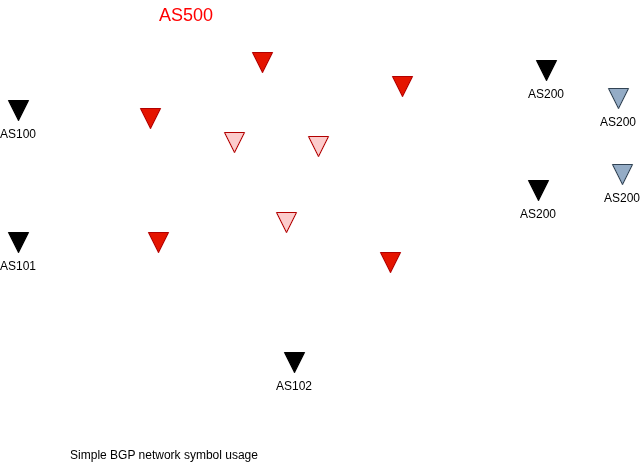
\includegraphics[width=0.7\linewidth]{bgp2.png} % https://drive.google.com/file/d/1EccfKdXZZyW0LT6cPnmi5AjUfwFKyOSz
    \caption{BGP example network}
    \label{fig:diag1}
\end{figure}

In this minimal diagram, there are only the core elements - BGP speakers. Border routers (ASBRs) are shown in strong colours, while internal IBGP-only peers are shown as pale.  Where needed, an AS number is attached to a BGP speaker, but generally colour is sufficient to distinguish AS membership.  The `missing elements' in this diagram are the peering links; a few links are added in the next diagram:\ref{fig:diag2}.  But notice that even in this quite `simple' network, showing all of the internal BGP links would be tedious and unhelpful.  So, in general, the existence of IBGP links is left implied, except in cases where it aids the argument.

\begin{figure}[H]
    \centering
    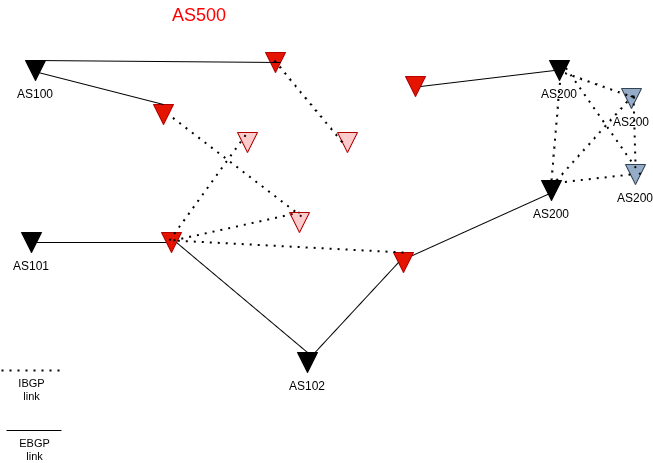
\includegraphics[width=0.7\linewidth]{bgp3.png}
    \caption{BGP example network - with some peer links}
    \label{fig:diag2}
\end{figure}

Here is a simpler, complete, network, showing the usually suppressed IBGP links:
\begin{figure}[H]
    \centering
    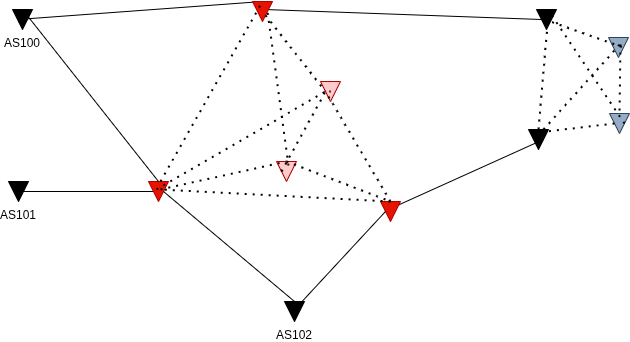
\includegraphics[width=0.7\linewidth]{bgp4.png} % https://drive.google.com/file/d/16C6qxZ84SvLd6x6U58ob4-CbPgehXUmq
    \caption{simpler BGP network, showing all peer links}
    \label{fig:diag3}
\end{figure}


\bigskip

For completeness, the more complex network of Figure \ref{fig:diag3} is presented again below, in Figure \ref{fig:diag4}, restructured using route reflection to reduce the number of BGP peering links.  Note that the difference between these networks,  Figure \ref{fig:diag3} and  Figure \ref{fig:diag4}, is only visible externally, and significant from a BGP configuration and state level - as routing systems they behave identically. `

\begin{figure}[H]
    \centering
    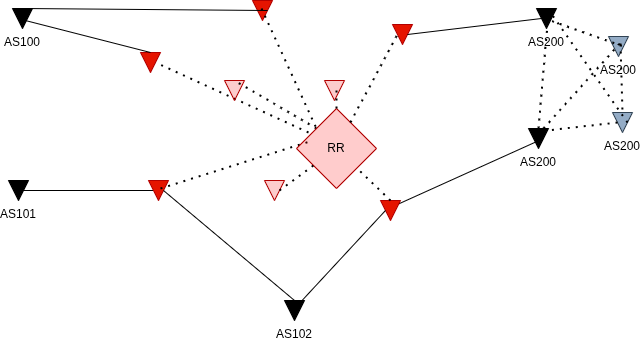
\includegraphics[width=0.7\linewidth]{bgp5.png}
    \caption{fully graphed BGP network, with Route Reflector}
    \label{fig:diag4}
\end{figure}

In all of these diagrams the network links shown represent only signalling connections, although in the case of \ref{fig:diag3} there is a one-to-one relation between  user-plane links and control-plane links, and likely even one-to-one relation to physical links.\footnote{In general, in larger AS systems, the IBGP associations are not direct, because the end-to-end paths between ASBRs are indirect.  Otherwise, there would be no need for either core routers, or even any IGP, e.g., OSPF, IS-IS, \ldots. \\
In contrast, EBGP links are almost invariably direct, both at signalling and forwarding plane level (IXP Route Servers excepted).}

But in fact the core AS in \ref{fig:diag4} will surely have L2 forwarding connections between every node, and also internal routing associations (OSPF or IS-IS) between all such connected nodes.

Note that there is no ambiguity whatsoever to these diagrams, even when no IBGP links are shown, in any cases, with or without Route Reflectors.

